% Created 2014-01-20 Mon 12:50
\documentclass[12pt]{article}
\usepackage[utf8]{inputenc}
\usepackage[T1]{fontenc}
\usepackage{amsmath,tikz}
\usepackage{amssymb,natbib}
\usepackage{hyperref,setspace}
\onehalfspacing

\usepackage{amsthm}

\newtheorem{lemma}{Lemma}

\title{One-dimensional screening: the non-linear pricing model}
\author{Christoph Schottmüller}
\date{\today}
\usepackage[margin=2.5cm]{geometry}



\begin{document}

\maketitle

\section{Model}
\label{sec:model}

A monopolist seller can produce a quantity $q\in\Re_+$ at costs $c(q)$ where $c$ is an increasing and convex function. There is a single buyer whose valuation for quantity $q$ is denoted by $v(q,\theta) $ where $v$ is assumed to be three times continuously differentiable.\footnote{I use ``valuation'' and ``willingness to pay'' interchangeably. In particular the payoff of a buyer of type $\theta $ when buying quantity $q$ at price $p$ is $v(q,\theta )-p$, i.e. utility is assumed to be ``quasi-linear''.}  Here $\theta $ denotes the consumer's ``type'' -- which is private information of the consumer and not known by the seller. From the seller's point of view, the type is distributed according to some distribution $F$ with continuous density $f$ on the support $[0,1]$.

It is furthermore assumed that $v_q>0$ (``more is better'') and $v_{q\theta }>0$ (``higher types have a higher marginal utility'') as well as $v(0,q)=0$ (``zero valuation for zero quantity'').  The assumption $v_{q\theta }>0$ is well known under different names (``single crossing condition'', ``Spence-Mirrlees condition'', ``constant sign condition''). This condition will play a major role in the proof of lemma \ref{lem:mon} below.

As the seller does not know the buyer's type, he will offer a whole ``menu'' of choices. A menu is a list of price-quantity pairs from which the consumer chooses one (which means that he gets the chosen quantity and has to pay the corresponding price). Put differently, the seller offers a price function which gives for every quantity the consumer might want, the price he has to pay.

The task is now to find the price function (or the menu) that maximizes expected profits.

\section{Revelation principle}
\label{sec:revelation-principle}

The first step, in this derivation is to apply the famous revelation principle which implies in this setting that it is without loss of generality to concentrate on menus $(q(\cdot),t(\cdot ))$, where $q(\theta )$ is the quantity a type $\theta $ receives and $t(\theta )$ is the price a type $\theta $ pays, which are ``incentive compatible'' and satisfy the ``participation constraint''. Incentive compatibility means that every type $\theta \in[0,1]$ finds it optimal to truthfully announce/reveal $\theta $ if he is faced with the following problem: ``Tell me a type $\hat{\theta }\in[0,1]$ and you will then get quantity $q(\hat{\theta })$ but you will have to pay $t(\hat{\theta })$.'' Individually rationality meand that $v(q(\theta ),\theta )-t(\theta )\geq 0$, i.e. every type is at least as well off consuming $q(\theta )$ at price $t(\theta )$ as he would be when consuming nothing at price 0.

You may have expected to try to find an optimal function $p(q)$ that assigns to every quantity a price but it turns out that the problem of finding the optimal $q(\theta )$ and $t(\theta )$ that satisfy the constraints of incentive compatibility and the participation constraint is mathematically simpler. The revelation principle tells us that the two problems are interchangeable. If you think a bit about it, that is actually not that surprising: Take some function $p(q)$. If the buyer has to choose from this function, every type will have some optimal choice $q^*(\theta )$ and he will pay price $p(q^*(\theta ))$. If we define, $q(\theta )=q^*(\theta )$ and $t(\theta ) = p(q^*(\theta ))$, then we have functions $q$ and $t$ that yield the same outcome as the $p(q)$ with which we started and are incentive compatible (think for a minute about it if incentive compatibility is not clear).\footnote{We can ensure that the participation constraint holds by adding the point $(0,0)$ to the menu.}

Finally, let us be a bit more precise what incentive compatibility means mathematically. I will call a pair of functions $q(\theta )$ and $t(\theta )$ -- each mapping from $[0,1]$ to $\Re_+$ -- a ``direct revelation mechanism''. Such a direct revelation mechanism is incentive compatible if for every $\theta \in[0,1]$ and every $\hat\theta\in[0,1]$ the inequality
$$v(q(\theta ),\theta )-t(\theta )\geq v(q(\hat\theta ),\theta )-t(\hat\theta)$$
holds. (The left hand side is the payoff of a type $\theta $ getting quantity $q(\theta )$ while paying $t(\theta )$. The right hand side is the payoff of a type $\theta $ getting quantity $q(\hat{\theta })$ and paying $t(\hat{\theta })$.) The direct revelation mechanism satisfies the participation constraints if the inequality
$$v(q(\theta ),\theta )-t(\theta )\geq 0$$
holds for all types $\theta \in[0,1]$.

Our task is therefore to maximize expected profits, namely
$$\int_0^1 [t(\theta )-c(q(\theta ))]f(\theta )\;d\theta $$
subject to the participation and incentive compatibility constraints. Here you will realize that we run into a problem: we have infinitely many constraints! (recall that for each $\theta $ and each $\hat{\theta }$ we have one incentive compatibility constraint\dots). To deal with this, we need to do something clever. What we will show is that a direct revelation mechanism is incentive compatible if and only if it satisfies two conditions (which are a bit simpler than the original incentive compatibility constraints):
\begin{enumerate}
\item an ``envelope condition'' (defined below)
  \item a monotonicity constraint, namely $q(\theta )$ has to be weakly higher for higher types.
\end{enumerate}

\section{Deriving the envelope and monotonicity condition}

Now, take a direct revelation mechanism consisting of the two functions $q(\theta )$ and $t(\theta )$ and \emph{for now assume} that it is  incentive compatible. We define $U(\theta )=v(q(\theta ),\theta )-t(\theta )$. As the mechanism is incentive compatible, the following holds for any two types $\theta '$ and $\theta ''$:
\begin{eqnarray*}
  v(q(\theta' ),\theta' )-t(\theta' )&\geq&v(q(\theta'' ),\theta' )-t(\theta'' )\\
v(q(\theta'' ),\theta'' )-t(\theta'' )&\geq&v(q(\theta' ),\theta'' )-t(\theta' ).
\end{eqnarray*}
These two conditions can be rewritten as 
\begin{eqnarray*}
  U(\theta ')&\geq&U(\theta '') -v(q(\theta ''),\theta '')+v(q(\theta ''),\theta ')\\
U(\theta'' )&\geq&U(\theta ') -v(q(\theta '),\theta ')+v(q(\theta '),\theta '').
\end{eqnarray*}
Rearranging these two inequalities gives 
\begin{eqnarray*}
  U(\theta ')-U(\theta '')&\geq& -v(q(\theta ''),\theta '')+v(q(\theta ''),\theta ')\\
U(\theta ')-U(\theta'' )&\leq& v(q(\theta '),\theta ')-v(q(\theta '),\theta '').
\end{eqnarray*}
Assume $\theta '>\theta ''$. Then combining these two inequalities gives
\begin{equation}
  \label{eq:1}
 \frac{ v(q(\theta ''),\theta ')-v(q(\theta ''),\theta '')}{\theta '-\theta ''} \leq \frac{ U(\theta ')-U(\theta '')}{\theta '-\theta ''}\leq \frac{ v(q(\theta '),\theta ')-v(q(\theta '),\theta '')}{\theta '-\theta ''}.
\end{equation}
Now we derive the monotonicity constraint: 
\begin{lemma}\label{lem:mon}
  In every incentive compatible mechanism, $\theta '>\theta ''$ implies $q(\theta ')\geq q(\theta '').$ 
\end{lemma}
\textbf{Proof. }(\ref{eq:1}) implies that 
\begin{equation*}
v(q(\theta ''),\theta ')-v(q(\theta ''),\theta '')\leq v(q(\theta '),\theta ')-v(q(\theta '),\theta '')
\end{equation*}
(recall that $\theta '-\theta ''>0$ by assumption). The last inequality can be rewritten as
\begin{equation*}
  \int_{\theta ''}^{\theta '}v_\theta (q(\theta ''),x)\,dx\leq \int_{\theta ''}^{\theta '}v_\theta (q(\theta '),x)\,dx
\end{equation*}
which in turn is equivalent to 
\begin{equation*}
0\leq \int_{q(\theta '')}^{q(\theta ')}\int_{\theta ''}^{\theta '}v_{q\theta} (y,x)\,dx\,dy.
\end{equation*}
By the assumption $v_{q\theta }>0$, the integrand of the previous expression is strictly positive everywhere. But then the previous inequality can (by $\theta ''<\theta '$) hold only if $q(\theta '')\leq q(\theta ')$. (Remember that $\int_a^b\dots=-\int_b^a\dots$.)

Since the types $\theta '$ and $\theta ''$ were arbitrary we get that $q$ has to be monotone, i.e. higher types lead to (weakly) higher decision.\qed

Next, we derive the envelope condition. In (\ref{eq:1}), the right hand side converges to $v_\theta (q(\theta '),\theta ')$ as $\theta ''\rightarrow\theta '$. If $q$ is continuous at $\theta '$, then the left hand side converges to $v_\theta (q(\theta '),\theta ')$ as well. This, of course, implies that the middle term also converges to $v_\theta (q(\theta '),\theta ')$. As the middle term is $U'(\theta )$, we then get $U'(\theta )=v_\theta (q(\theta '),\theta ')$. 
 
As $q$ is monotone (see the lemma above), $q$ is continuous almost everywhere.\footnote{This useful fact follows from the following idea: At every discontinuity $q$ has to ``jump'' over a rational number. If a monotone, say increasing, function had an uncountable number of discontinuities we would therefore have to conclude that there are uncountably many rational numbers (as the function is monotone it has to jump over a different rational at every discontinuity). The rational numbers, however, are countable.  } Consequently, we have shown the following result:
\begin{lemma}[envelope theorem]
  In an incentive compatible mechanism, $U'(\theta )=v_\theta (q(\theta ),\theta )$ for almost all $\theta \in\Theta $ and therefore\footnote{Here we use the fundamental theorem of calculus. Strictly, speaking we have not checked its conditions properly. In particular, we have to verify that $v_\theta (q(\theta ),\theta )$ is bounded and integrable. Without going into details, let me just say that given the assumptions made this can be shown by showing that for $q$ a bounded domain can be used without loss of generality.}
  \begin{equation}\tag{envelope condition}
    U(\theta )=U(0)+\int_0^\theta v_\theta (q(x),x)\,dx.
  \end{equation}
\end{lemma}

We have now established that incentive compatibility implies both the monotonicity and the envelope condition. Now we want to show the reverse: If a mechanism satisfies both the monotonicity and the envelope condition, then this mechanism is incentive compatible.

Let $t$ and $q$ be such that the envelope condition and monotonicity are satisfied. Take arbitrary types $\theta '$ and $\theta ''$. Because $v_{q\theta }>0$, monotonicity of $q$ implies that
\begin{equation}\label{eq:3}
  \int_{\theta ''}^{\theta '}\int_{q(\theta '')}^{q(x)}v_{q\theta }(y,x)\,dy\,dx\geq 0.
\end{equation}
(The trick is that monotonicity implies $q(x)\geq q(\theta '')$ for all $x\in[\theta '',\theta ']$ if $\theta '>\theta ''$. If $\theta '<\theta ''$, then we can rewrite the expression above as $\int_{\theta '}^{\theta ''}\int^{q(\theta '')}_{q(x)}v_{q\theta }(y,x)\,dy\,dx\geq 0$ and monotonicty implies then that $q(x)\leq q(\theta '')$ for all $x\in[\theta ',\theta '']$.) 

Rewriting (\ref{eq:3}) gives
\begin{equation*}
  \int_{\theta ''}^{\theta '}v_{\theta }(q(x),x)-v_{\theta }(q(\theta ''), x)\,dx\geq 0.
\end{equation*}
By the envelope condition $\int_{\theta ''}^{\theta '}v_{\theta }(q(x),x)\,dx=U(\theta ')-U(\theta '')$, and therefore the previous expression is equivalent to
\begin{equation*}
  U(\theta ')-U(\theta '')-v(q(\theta ''),\theta ')+v(q(\theta ''),\theta '')\geq 0.
\end{equation*}
Rearranging gives 
\begin{equation*}
  U(\theta ')\geq U(\theta '')+v(q(\theta ''),\theta ')-v(q(\theta ''),\theta '')=v(q(\theta ''),\theta ')-t(\theta '').
\end{equation*}
But this is exactly the incentive compatibility conditions for $\theta '$ and $\theta ''$. Since $\theta '$ and $\theta ''$ were arbitrary, the mechanism is incentive compatible which is what we wanted to show.

Hence, we conclude that incentive compatibility is equivalent to envelope condition and monotonicity condition. In our profit maximization problem we can use envelope and monotonicity condition as constraints instead of the infinite number of incentive compatibility conditions.

\section{Profit maximization}
\label{sec:profit-maximization}

Note that -- by plugging in the definition of $U(\theta )$ -- we can express expected profits also as
$$\int_0^1 [v(q(\theta ),\theta )-c(q(\theta ))-U(\theta )]f(\theta )\;d\theta. $$
(Verbally: profits are welfare minus the ``rent'' of the buyer.) As the envelope condition is stated in terms of $U$ rather than $t$, we will use this form where we substitute out $t$ and choose $U$ instead. We can later use the definition of $U$ to get $t$ as soon as we know $U$ and $q$.

Our profit maximization problem, therefore reads
$$\max_{q(\cdot),U(\cdot)} \int_0^1 [v(q(\theta ),\theta )-c(q(\theta ))-U(\theta )]f(\theta )\;d\theta. $$
subject to the constraints
\begin{itemize}
\item $U(\theta )=U(0)+\int_0^\theta v_\theta (q(x),x)\,dx$ (envelope condition)
\item $q$ is weakly increasing (monotonicity constraint)
  \item $U(\theta )\geq 0$ for all $\theta \in[0,1]$ (participation constraint).
\end{itemize}

To simplify matters, we first plug the envelope constraint into our objective which yields:

$$\max_{q(\cdot),U(0)} \int_0^1 [v(q(\theta ),\theta )-c(q(\theta ))-U(0)-\int_0^\theta v_\theta (q(x),x)\,dx]f(\theta )\;d\theta $$
subject to participation and monotonicity constraint. Admittedly, the objective is a bit ugly as it includes an integral inside an integral. We use a small aside (using integration by parts to simplify):\footnote{The ``parts'' are (i) $\int_0^{\theta} v_\theta (q(x),x)\,dx$ and (ii) $f(\theta )$. To take the derivative of the first part with respect to $\theta $, recall that a derivative of an integral with respect to its upper boundary is the integrand evaluated at the upper boundary.}
\begin{multline*}
  \int_0^1\int_0^\theta v_\theta (q(x),x)\,dx\,f(\theta )\,d\theta =\left[\int_0^\theta v_\theta (q(x),x)\,dx\,F(\theta )\right]_0^1-\int_0^1v_\theta (q(\theta ),\theta ) F(\theta )\;d\theta\\
  =\int_0^1 v_\theta (q(x ),x )\,dx*1 -\int_0^1v_\theta (q(\theta ),\theta ) F(\theta )\;d\theta\\
  =\int_0^1(1-F(\theta ))v_\theta (q(\theta ),\theta )\;d\theta 
\end{multline*}

This allows us to rewrite our profit maximization problem once more as 
$$\max_{q(\cdot),U(0)} \int_0^1 [v(q(\theta ),\theta )-c(q(\theta ))-U(0)-\frac{1-F(\theta )}{f(\theta )}v_\theta (q(\theta ),\theta )]f(\theta )\;d\theta $$
subject to participation constraint and monotonicity constraint. Now given this objective clearly we want to choose $U(0)$ as low as possible. By the participation constraint, however, we cannot choose a negative $U(0)$. Hence, the optimal $U(0)$ has to be 0.

This leaves us with the maximization problem
$$\max_{q(\cdot)} \int_0^1 [v(q(\theta ),\theta )-c(q(\theta ))-\frac{1-F(\theta )}{f(\theta )}v_\theta (q(\theta ),\theta )]f(\theta )\;d\theta $$
subject to the monotonicity constraint.

The final trick will look a bit weird but it is in fact the standard way to proceed in the literature: We will ignore the monotonicity constraint and later find assumptions under which this constraint is not binding and can therefore be ignored.\footnote{Yes, it is possible to solve problems where the monotonicity constraint is binding. However, this is mathematically not so easy and beyond the scope of this course. Consult \cite[ch. 2.3.3]{bolton2005contract} if you want to know a bit more.}

Of course, even this leaves us with the daunting task of choosing the function $q$ that maximizes $\int_0^1 [v(q(\theta ),\theta )-c(q(\theta ))-\frac{1-F(\theta )}{f(\theta )}v_\theta (q(\theta ),\theta )]f(\theta )\;d\theta$. However, this problem is much simpler than it might look at first. The solution is to maximize the integrand ``pointwise'', i.e. for each $\theta $ we choose the $q(\theta )$ that maximizes $[v(q(\theta ),\theta )-c(q(\theta ))-\frac{1-F(\theta )}{f(\theta )}v_\theta (q(\theta ),\theta )]f(\theta )$.\footnote{If this appears strange, think about a simpler problem, say $\max_{q_1,q_2,q_3} a_1(q_1)*f(1)+a_2(q_2)*f(2)+a_3(q_3)*f(3)=\max_{q_1,q_2,q_3}\sum_{i=1}^3a_i(q_i)f(i)$ where $a_1$, $a_2$ and $a_3$ are some functions and $f(1),f(2),f(3)>0$ are some weights. Clearly, you will choose the $q_1$ that maximizes $a_1$, the $q_2$ that maximizes $a_2$ and the $q_3$ that maximizes $a_3$ -- each $q_i$ affects a different part of the sum and therefore the maximization problem can be separated into three independent sub-problems. We are doing the same with the integral\dots just that we have an integral instead of a sum. But, if you remember high-school mathematics, you might recall that an integral is simply the limit of a sum (I like to call an integral a ``fancy sum'' though this is admittedly a bit loose) and therefore there is actually not much of a difference between the simple problem and the optimization problem in the main text.} The solution has therefore to satisfy the first order condition
\begin{equation}
v_q(q(\theta ),\theta )-c_q(q(\theta ))-\frac{1-F(\theta )}{f(\theta )}v_{q\theta }(q(\theta ),\theta )=0.\label{eq:2}
\end{equation}

Finally, I want to state some assumptions under which (i) the first order condition has a unique solution and therefore defines the optimal $q(\theta )$ and (ii) the neglected monotonicity constraint does not bind. As for (i), we can assume $v_{qq}< 0$ and $v_{qq\theta }\leq 0$ which implies together with the convexity of $c$ that the maximization problem is strictly concave. For (ii), it is customary to assume that $F$ is a distribution for which $f(\theta )/(1-F(\theta ))$ (the so called ``hazard rate'') is non-decreasing (this is true for the uniform, the normal and many other distributions) and $v_{q\theta \theta }\geq 0$. If you apply the implicit function theorem to the first order condition (\ref{eq:2}), these assumptions guarantee that the implicitly defined solution $q(\theta )$ is strictly increasing.\footnote{Alright, if you really want to see it: the implicit function theorem yields
$$q'(\theta )=-\frac{v_{q\theta }-\frac{1-F}{f}v_{q\theta \theta }-\frac{d\frac{1-F}{f}}{d\theta }v_{q\theta }}{v_{qq}-c_{qq}-\frac{1-F}{f}v_{qq\theta }}$$ where I left out the arguments of the functions for better readability. Our assumptions ensure that all terms in the numerator are non-negative (and the first one is strictly positive) while all terms in the denominator are non-positive (with the first one being strictly negative). With the minus in front, the fraction is therefore strictly positive.}

\section{Bringing it finally together}
\label{sec:bringing-it-finally}

Now, under our new assumptions, equation (\ref{eq:2}) implicitly defines the optimal $q(\theta )$. By plugging this optimal $q(\theta )$ into the envelope condition (and recall that $U(0)=0$), we get $U(\theta )$ in the optimal menu. From the definition of $U$, i.e. $U(\theta )=v(q(\theta ),\theta )-t(\theta )$, we can then calculate $t(\theta )$. And there we go: we have the menu maximizing expected profits!

Ok, you are still not happy and want the optimal price schedule $p(q)$. Well easy: For every $\bar q$ such that $q(\theta' )=\bar q$ for some type $\theta' \in[0,1]$, the price is $t(\theta' )$.\footnote{For all other quantities (i.e. those bought by no type in the optimal menu), we charge a price sufficiently high that no type would eve want to buy these quantities.}

\subsection{A numerical example}
\label{sec:an-example}

All of this is probably easier if we use an example. Let's say $v(q,\theta )=(1+\theta )\sqrt{q}$, $c(q)=q$ and let $F(\theta )=\theta $ (i.e. we use the uniform distribution on $[0,1]$). Check that indeed all our assumptions are satisfied then. The first order condition becomes then
$$\frac{1+\theta }{2\sqrt{q(\theta )}}-1-\frac{1-\theta }{1}\frac{1}{2\sqrt{q(\theta) }}=0$$
which can be solved for $q(\theta )$ as
$$q(\theta )=\theta ^2$$
which is clearly strictly increasing in $\theta $. Finally, $U(\theta )=\int_0^\theta \sqrt{q(x)}\,dx=\int_0^\theta x\,dx=\theta ^2/2$ which gives $t(\theta )=v(q(\theta ),\theta )-U(\theta )=(1+\theta )\sqrt{\theta ^2}-\theta ^2/2=\theta +\theta ^2/2$.

If one wants to derive the price function $p(q)$, note that quantity $q\in[0,1]$ is bought by type $\sqrt{q }$ and therefore the seller charges for quantity $q$ a price of $t(\sqrt{q})=\sqrt{q}+q/2$. We therefore get that $p(q)=\sqrt{q}+q/2$ for $q\in[0,1]$ (and prices are sufficiently high for $q>1$ so that no type wants to buy such high quantities).

\section{Some further remarks}
\subsection{ ``Single crossing'' and monotonicity: A graphical explanation}

The utility of type $\theta $ when getting quantity $q$ and paying price $t$ is $v(q,\theta )-t$. Think of the consumer's indifference curves in a $q,t$ diagram. Recall that an indifference curve are all the points $(q,t)$ such that $v(q,\theta )-t=\bar{U}$ for some constant $\bar{U}$. The slope of the indifference curve in a point $(q,t)$ is 
\begin{equation*}
  \left.\frac{d\,t}{d\,q}\right|_{U=\bar{U}}=v_q(q,\theta )
\end{equation*}
as can seen from rearranging the equation defining the indifference curve as $t=v(q,\theta )-\bar{U}$.
Intuitively, if we give the consumer one (marginal) unit more, then he is willing to pay $v_q(q,\theta )$ for this additional unit. Hence, we have to charge him $v_q(q,\theta )$ more if we want to keep him indifferent to the starting point.

The single crossing assumption $v_{q\theta }>0$ states that higher types have steeper indifference curves. That is, if the indifference curves of types $\theta '$ and $\theta ''<\theta '$ intersect in one point $(q',t')$ then the curve of $\theta '$ will be steeper and therefore intersect the curve of $\theta ''$ ``from below'' (that is the $\theta '$ curve is below (above) the curve of $\theta ''$ for lower (higher) $q$ than $q'$). Since this is true for any intersection, a given indifference curve of type $\theta '$ can intersect a given indifference curve of type $\theta ''$ only once: Suppose it intersected twice. By what we just said it would have to  intersect both times ``from below''. But as indifference curves are continuous,\footnote{Continuity of the indifference curves follows from the assumed continuity of $v$.} this implies that in between there must be an intersection ``from above''. An intersection from above is, however, impossible by $v_{q\theta }>0$. This contradicts that there is more than one intersection. This is where the name ``single crossing'' comes from.

\begin{figure}[h]
  \centering
  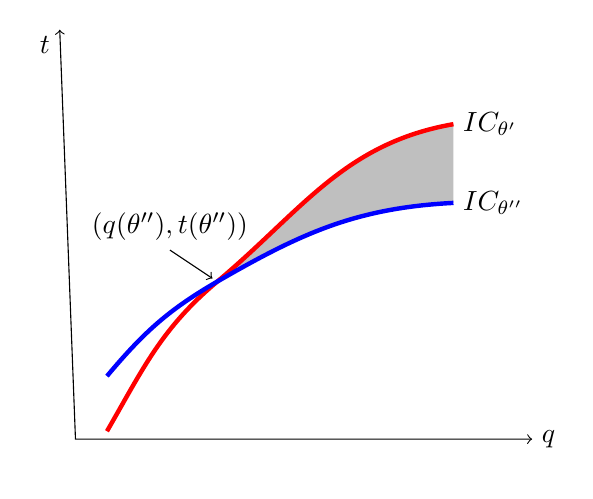
\begin{tikzpicture}[scale=2]
\draw[-] (-0.2,-0.2)--(-0.2,-0.2);
\draw[<->] (3,0)--(0.1,0)--(0,2.6);
\node[right] at  (3,0){$q$};
\node[left] at (0,2.5){$t$};
%\draw[domain=0.3:2.5,thick,blue] plot(\x,{sqrt(\x)});
\path[fill=lightgray, domain=1:2.5]  (1,1) to [out=40,in=190](2.5,2.0) -- (2.5,1.5) to [out = 183,in=30] (1,1);
\draw[ultra thick,red] (0.3,0.05) to [out=60,in=220] (1,1) to [out=40,in=190](2.5,2.0);
\draw[ultra thick,blue](0.3,0.4) to [out=50, in = 210](1,1) to [out=30, in = 183](2.5,1.5);
%\draw[domain=0.3:2.5,thick,red] plot(\x,{2*sqrt(\x)-1});

\node[above] at (.7,1.2){$(q(\theta''),t(\theta''))$};
\draw[->] (.7,1.2)--(.97,1.02);
\node[right] at (2.5,2.0){$IC_{\theta'}$};
\node[right] at (2.5,1.5){$IC_{\theta''}$};
\end{tikzpicture}
  \caption{Single crossing and monotonicity: Indifference curves of $\theta '$ and $\theta ''<\theta '$ through the contract $(q(\theta ''),t(\theta ''))$}
  \label{fig:mon}
\end{figure}

How does this help us to obtain our monotonicity result? In figure \ref{fig:mon} I draw the indifference curves of two types, $\theta ''$ and $\theta '$ with $\theta '>\theta ''$, passing through the contract $(q(\theta ''),t(\theta ''))$ intended for $\theta ''$. As $\theta '>\theta ''$, we have drawn the indifference curve of $\theta '$ -- labeled $IC_{\theta '}$ -- steeper than the indifference curve of $\theta ''$ -- labeled $IC_{\theta ''}$. (This is the role of the single crossing condition $v_{q\theta }>0$ in the figure.)

Where can the contract of type $\theta '$ be if we want the menu to be incentive compatible? In order to be incentive compatible, $\theta '$ has to prefer his own contract $(q(\theta '),t(\theta '))$ to $(q(\theta ''),t(\theta ''))$. Hence, $(q(\theta '),t(\theta '))$ has to be below $IC_{\theta '}$ (recall that right bottom is the direction which the consumer likes better in the $q,t$ diagram: get more, pay less). Incentive compatibility furthermore requires that $\theta ''$ prefers $(q(\theta ''),t(\theta ''))$ over $(q(\theta '),t(\theta '))$. Hence, $(q(\theta '),t(\theta '))$ has to be above $IC_{\theta ''}$. Taking these two requirements together, $(q(\theta '),t(\theta '))$ has to be in the shaded area in figure \ref{fig:mon}. Note that all points in the shaded area have a $q$ above $q(\theta '')$. Hence, $q(\theta ')\geq q(\theta '')$ for any incentive compatible menu -- we obtain the monotonicity condition.

\subsection{Some remarks on local and global incentive constraints}

Both envelope and monotonicity condition can be regarded as local constraints. That is, under the single crossing assumption, a type does not want to misrepresent as another type if and only if he does not want to misrepresent as a ``closeby'' type. Put differently, if we design a mechanism in which no type is able to benefit from an $\varepsilon $ deviation, then no type can gain froman arbitrary misrepresentation.

To see the local nature of the constraint it is useful to look at the special case in which the function $q$ is continuous and differentiable. In this case, monotonicity and envelope condition can be derived from the first and second order conditions for a local maximum in the optimization problem of the consumer:  The type announcement problem of type $\theta $ can be written as
\begin{equation*}
  \max_{\hat \theta }v(q(\hat{\theta }),\theta )-t(\hat{\theta }).
\end{equation*}
This problem has the first order condition $v_q(q(\hat\theta ),\theta )q_\theta (\hat \theta)-t_\theta (\hat{ \theta })=0$. In an incentive compatible mechanism, the optimal type announcement is the true type and therefore $v_q(q(\theta ),\theta )q_\theta ( \theta)-t_\theta ({ \theta })=0$. To get to the envelope condition, recall that $U(\theta )=v(q(\theta ),\theta )-t(\theta )$ and therefore $U'(\theta )=v_\theta (q(\theta ),\theta )+v_q(q(\theta ),\theta )q_\theta ( \theta)-t_\theta ({ \theta })$. By the first order condition, the difference of the last two terms is 0 in every incnetive compatible mechanism and we get $U'(\theta )=v_\theta (q(\theta ),\theta )$, i.e. the envelope condition.

To get the monotonicity condition, consider the second order condition for a maximum in the consumer's type announcement problem: $v_{qq}(q(\hat\theta ),\theta )q_\theta (\hat \theta)+v_{q}(q(\hat\theta ),\theta )q_{\theta \theta} (\hat \theta)-t_{\theta \theta} (\hat{ \theta })\leq0$ where the left hand side has to be evaluated at the optimum $\hat{\theta }=\theta $ (i.e. assuming incentive compatibility). By the previous paragraph, the first order condition $v_q(q(\theta ),\theta )q_\theta ( \theta)-t_\theta ({ \theta })=0$ holds for every type in an incentive compatible mechanism. Hence, the derivative with respect to $\theta $ of the left hand side has to be zero and we obtain $v_{q\theta }(q(\theta ),\theta )q_\theta (\theta )+v_{qq}(q(\theta ),\theta )q_\theta ( \theta)+v_{q}(q(\theta ),\theta )q_{\theta \theta} ( \theta)-t_{\theta \theta} ({ \theta })=0$. Plugging this back into the second order condition, the second order condition (evaluated at $\hat{\theta }=\theta $) becomes $-v_{q\theta }(q(\theta ),\theta )q_\theta (\theta )\leq 0$. By the assumption $v_{q\theta }>0$, this can only hold if $q_\theta (\theta )\geq 0$, i.e. the monotonicity constraint.

What we have shown is that in an incentive compatible mechanism the envelope and monotonicity constraint hold because they are equivalent to the first and second order condition for a \emph{local} maximum in the type announcement. The striking result that we showed in section 1 is that these two constraints are also sufficient for incentive compatibility, i.e. the conditions for a local maximum imply a global maximum in our type announcement problem. This property holds only under the single crossing condition $v_{q\theta }>0$. That is, if this condition is violated, then complicated non-local incentive constraints can be binding (e.g. type $0.5$ may be indifferent between his menu point and the menu point of type $0.3$ in the optimal mechanism). As this problem is much less tractable, solutions are known only for special cases, see \cite{araujo2010adverse} and \cite{schottmueller2015jet}.

\bibliographystyle{chicago}
\bibliography{/home/christoph/stuff/bibliography/references.bib}

\end{document}

